\documentclass[12pt]{article}

\usepackage[T1]{fontenc}
\usepackage{xcolor}
\usepackage{listings}
\usepackage{graphicx}

\begin{document}

\title{Tugas Database II}
\author{M. Farhan Fadlurrahman (1184072)}
\date{}
\maketitle

\section*{Membuat Data}
	\begin{enumerate}
		\item sebelumnya olah terlebih dahulu data yang didapat agar data yang dimasukan ke database tidak terjadi kesalahan dan redudansi.\\
		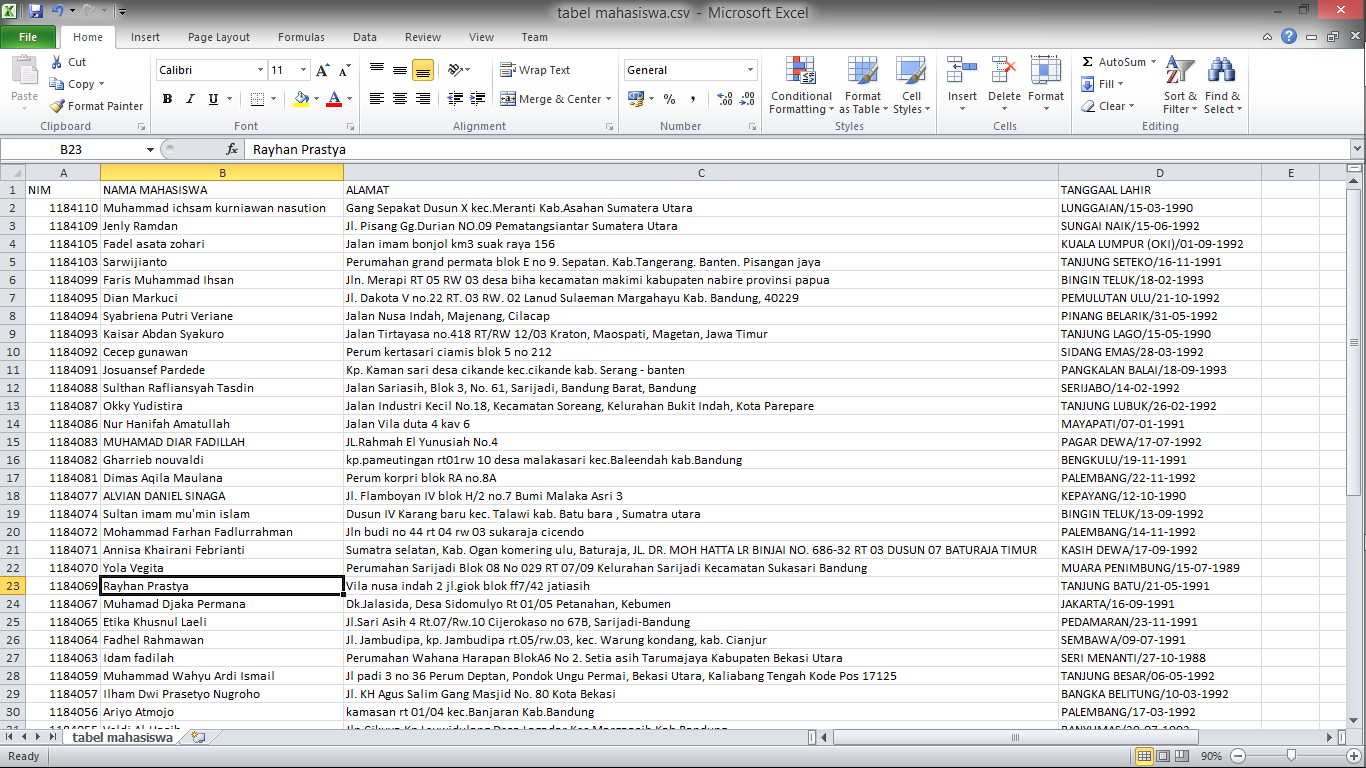
\includegraphics[scale=0.3]{src/21}
		
		\item pisahkan data menjadi beberapa tabel
		\item kemudian berikan kode pada setiap masingmasing data yang akan digunakan sebagai primary key.
		\item kemudian simpan data tersebut
	\end{enumerate}

\section*{Membuat Workspace}\
	\begin{enumerate}
		\item Untuk membaut workspace oracle pertama masuk website oracle untuk membuat workspace, kemudian klik "get started for free".\\
		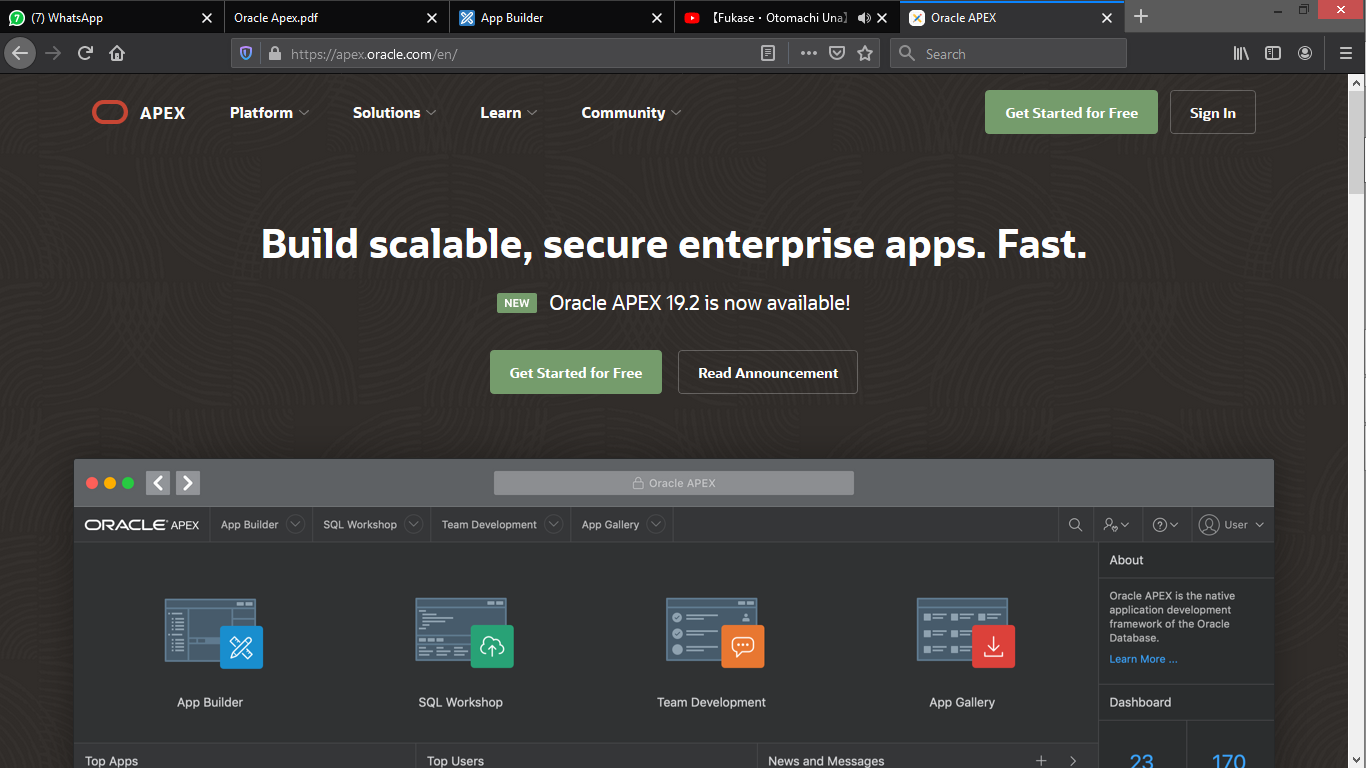
\includegraphics[scale=0.3]{src/1}
		\item Kemudian di halaman selanjutnya klik "request a free workspace".\\
		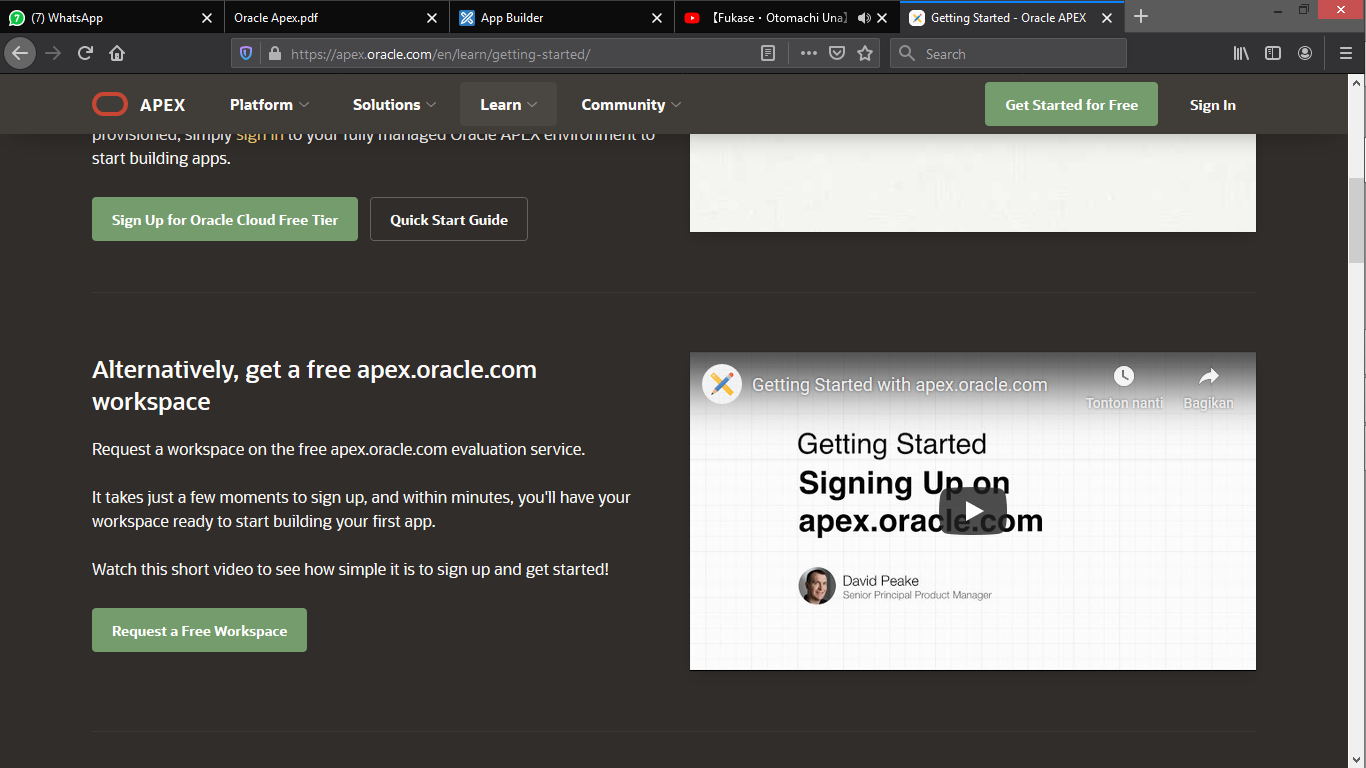
\includegraphics[scale=0.3]{src/2}
		\item Selanjutnya akan di arahkan ke halaman request a workspace, kemudian isi semua formulir sampai selesai.\\
		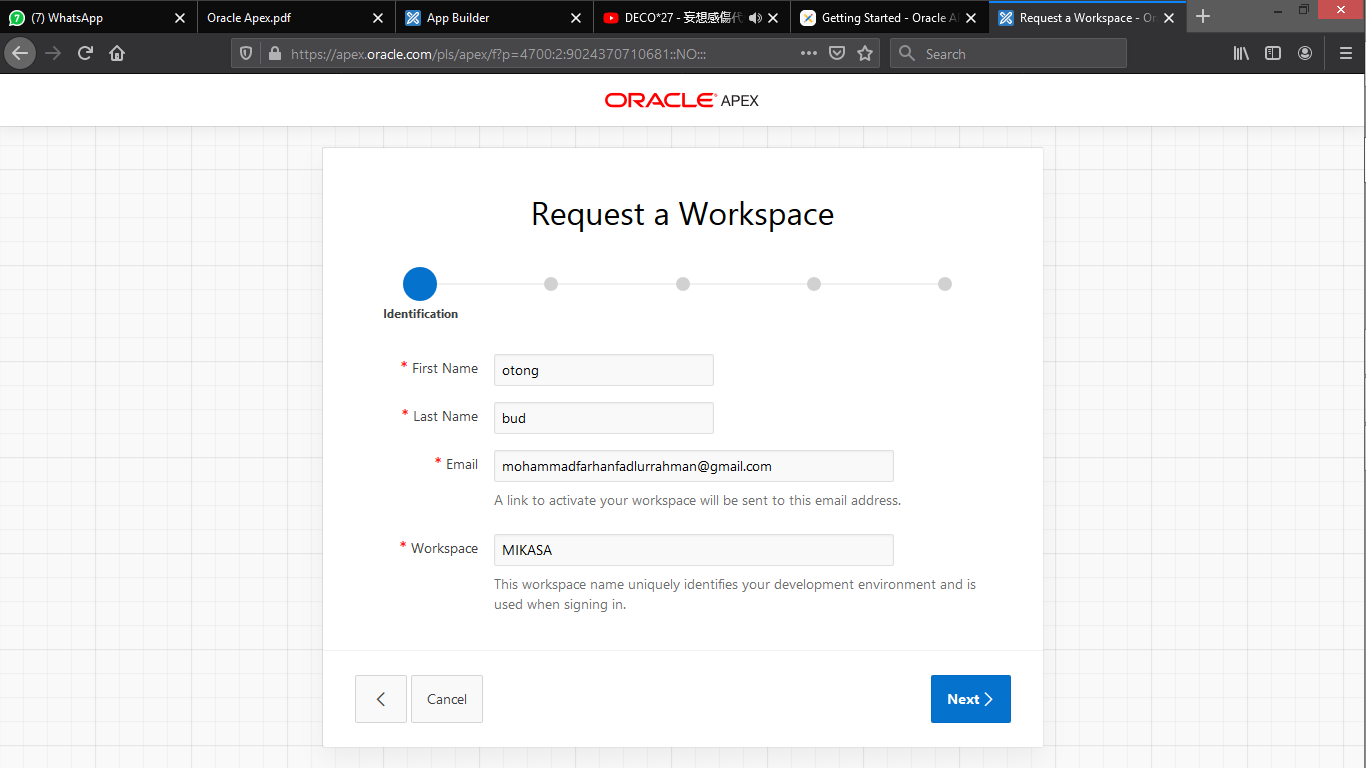
\includegraphics[scale=0.3]{src/3}
		\item Setelah mengisi formulir, oracle akan mengirimkan confirmasi verifikasi ke email yang di masukan, selanjutnya buka email yang di kirim oleh oracle kemudian klik "Create Workspace".\\
		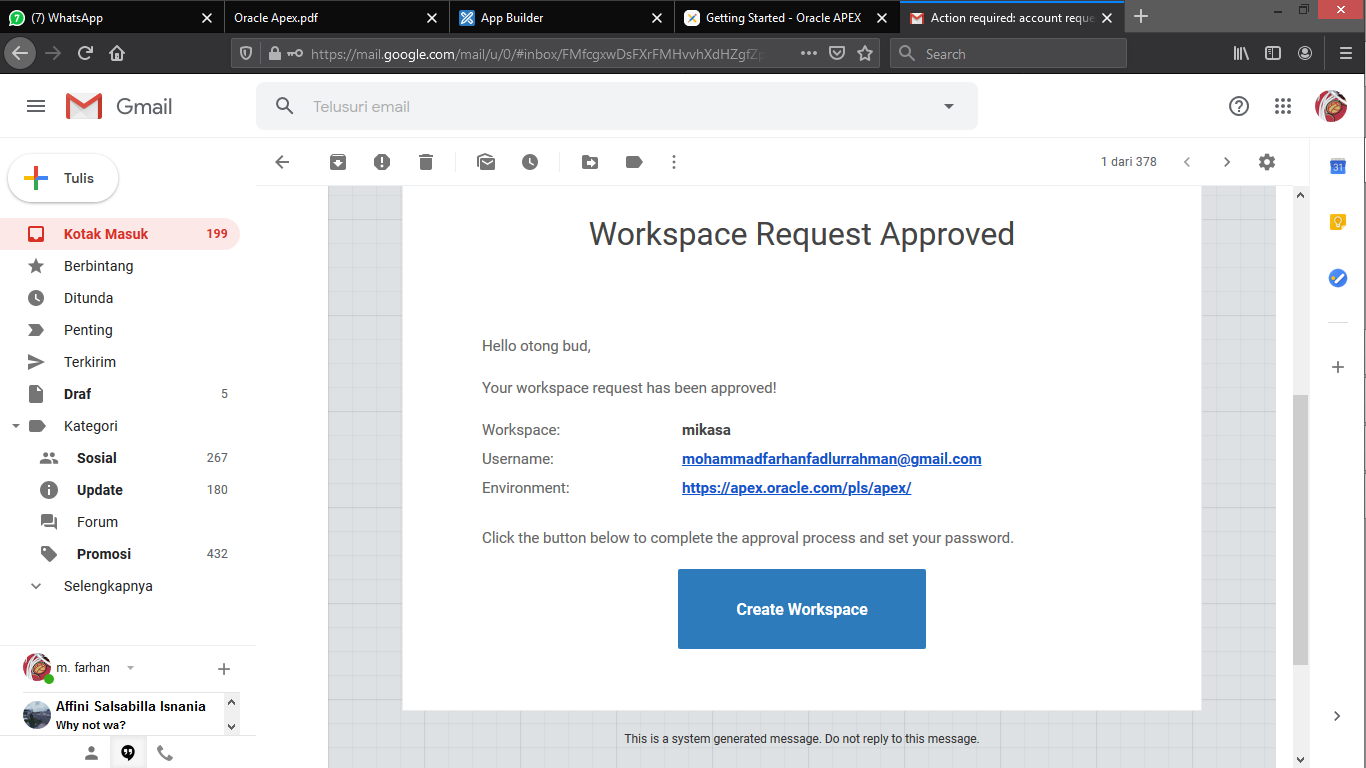
\includegraphics[scale=0.3]{src/4}
		\item selanjutnya workspace siap digunakan.\\
		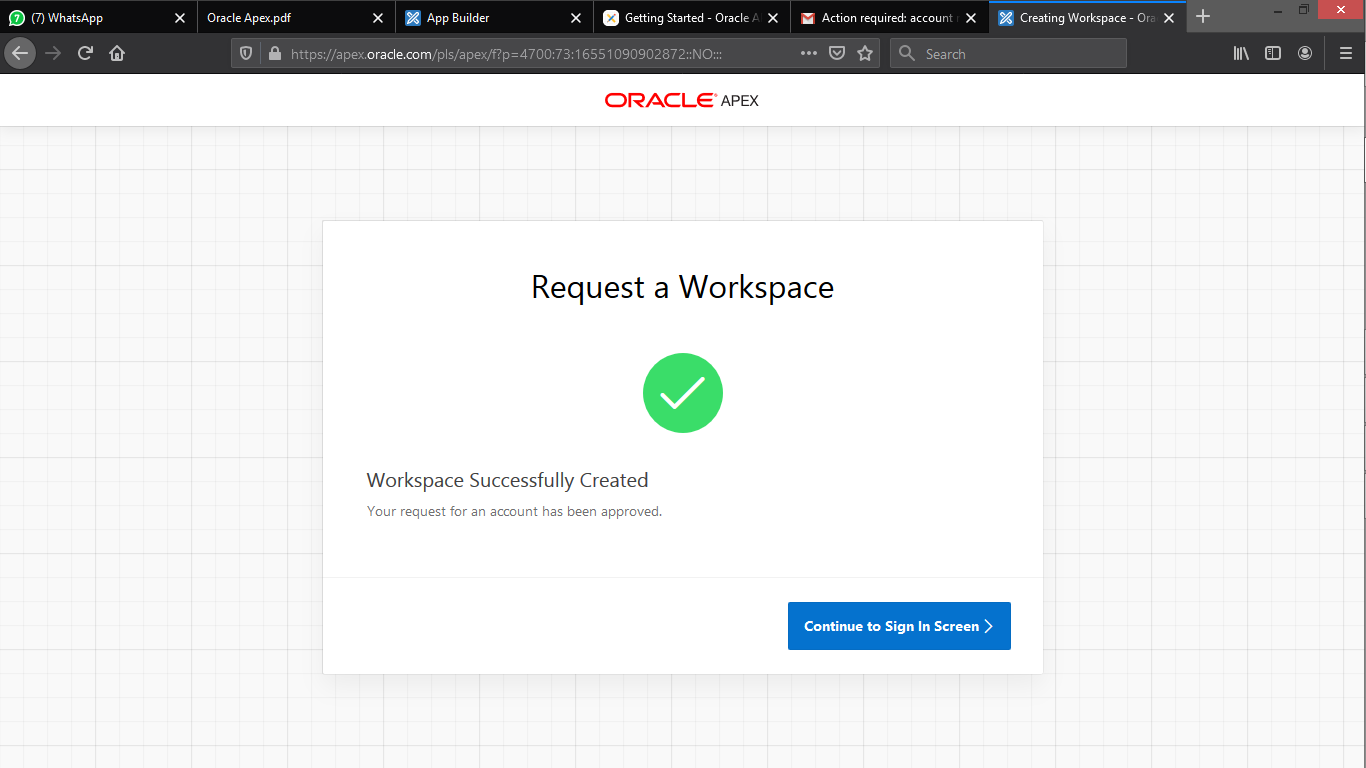
\includegraphics[scale=0.3]{src/5}
	
	\end{enumerate}
	
\section*{Membuat aplikasi}
	\begin{enumerate}
		\item Untuk membuat aplikasi pertama adalah siapkan dahulu file csv. kemudian didalam apex pilih "app builder"\\
		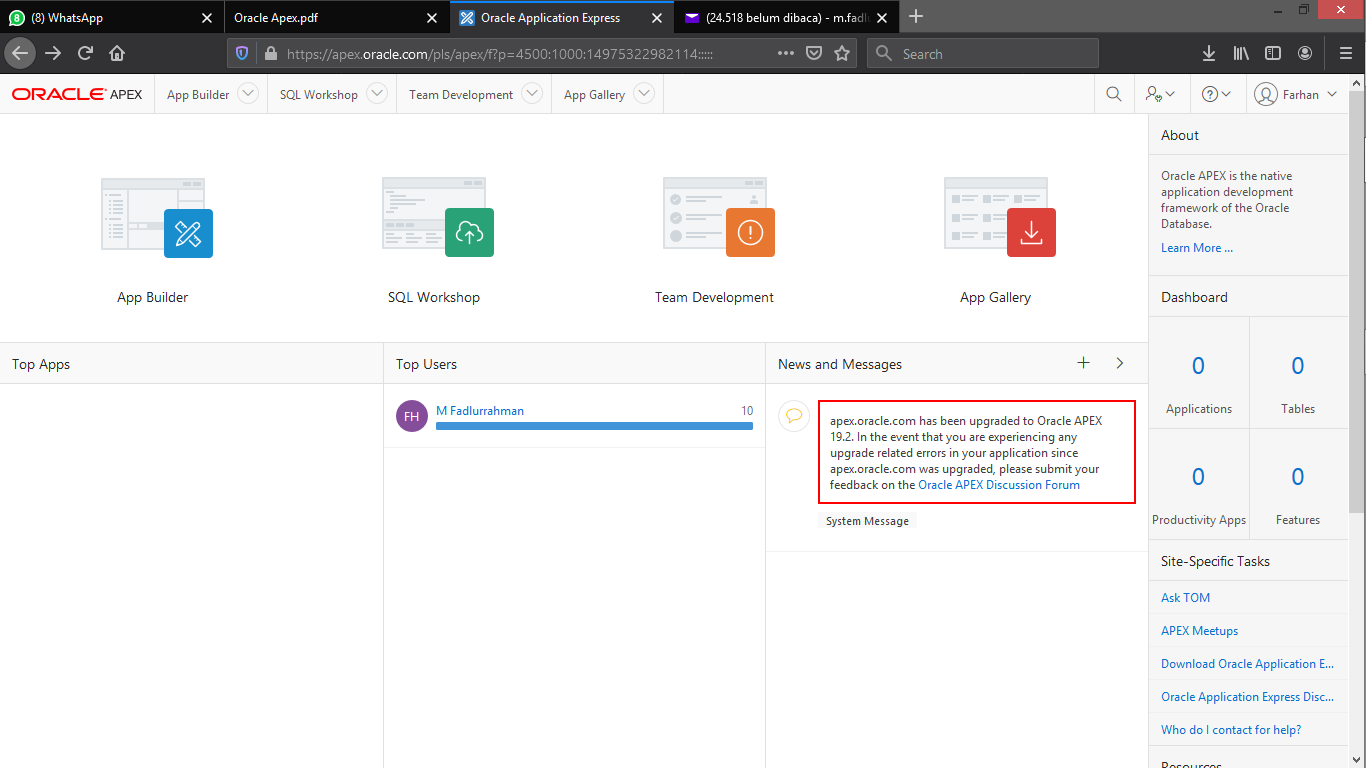
\includegraphics[scale=0.3]{src/6}
		\item Didalam app builder pilih "Create"\\
		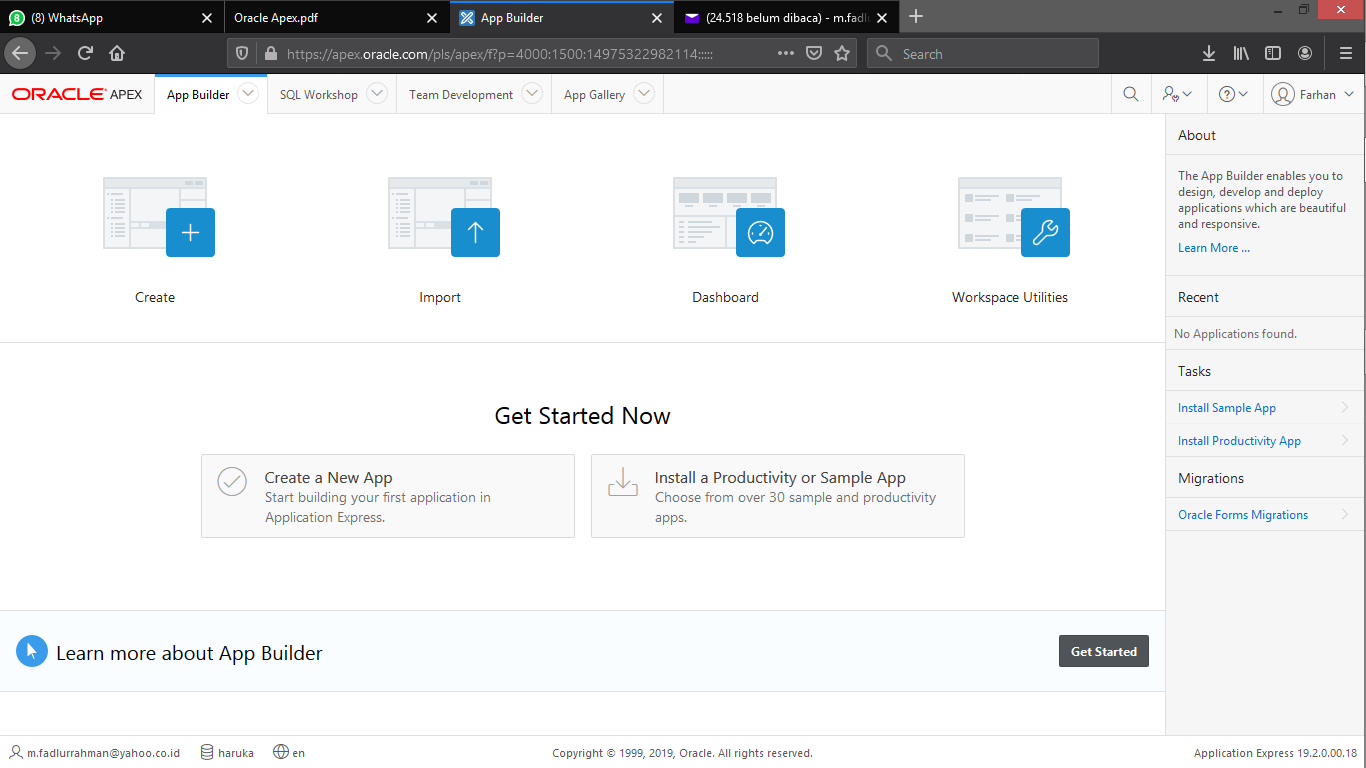
\includegraphics[scale=0.3]{src/7}
		\item Didalam Create pilih from a file untuk memilih file csv. yang telah di buat.\\
		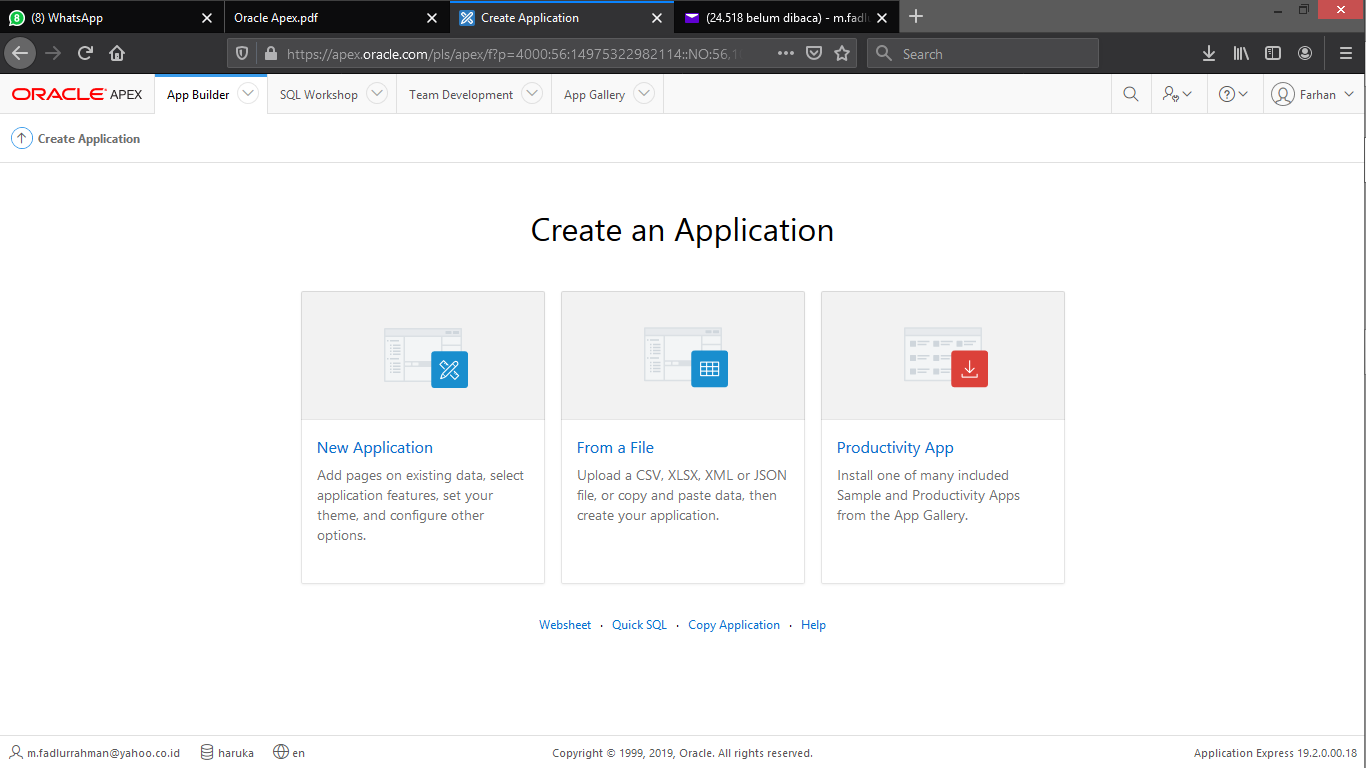
\includegraphics[scale=0.3]{src/8}
		\item Upload file csv. yang diinginkan\\
		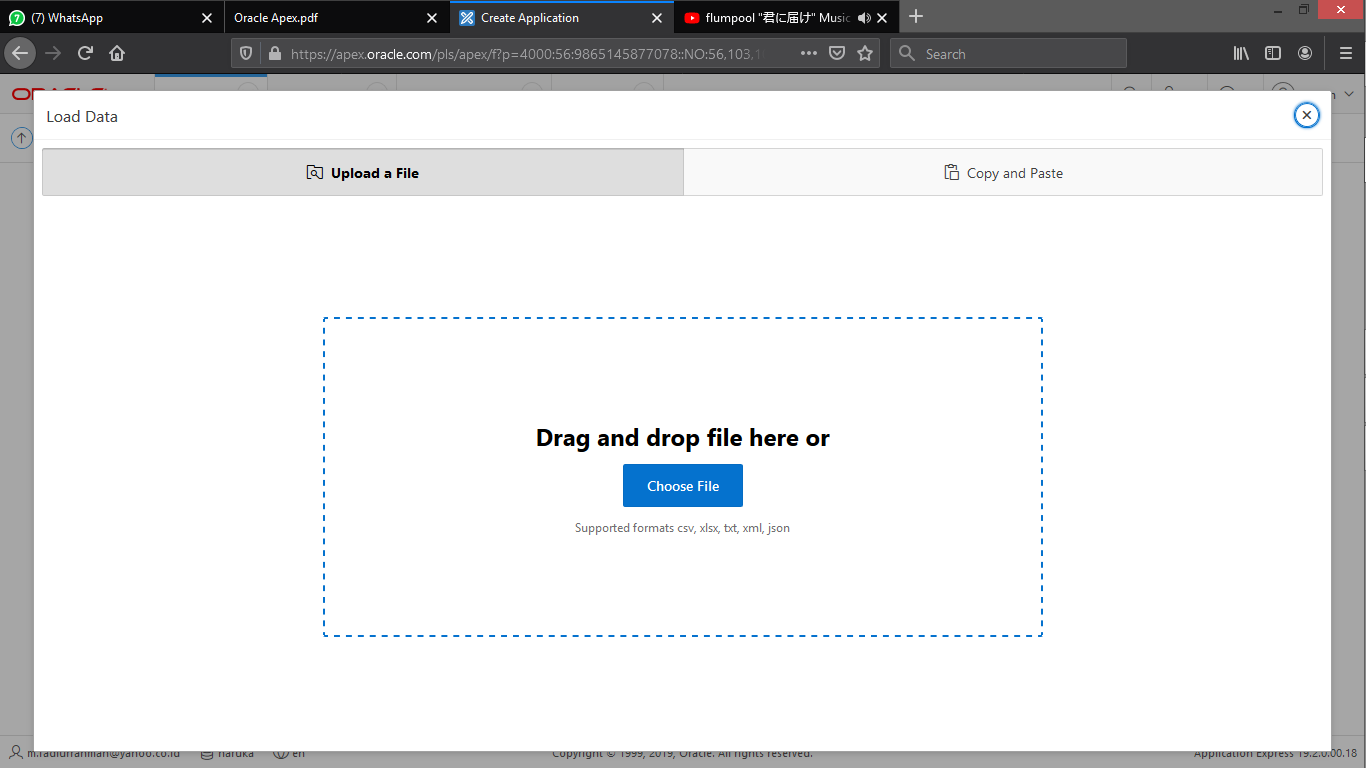
\includegraphics[scale=0.3]{src/9}
		\item Selanjutnya isi nama table\\
		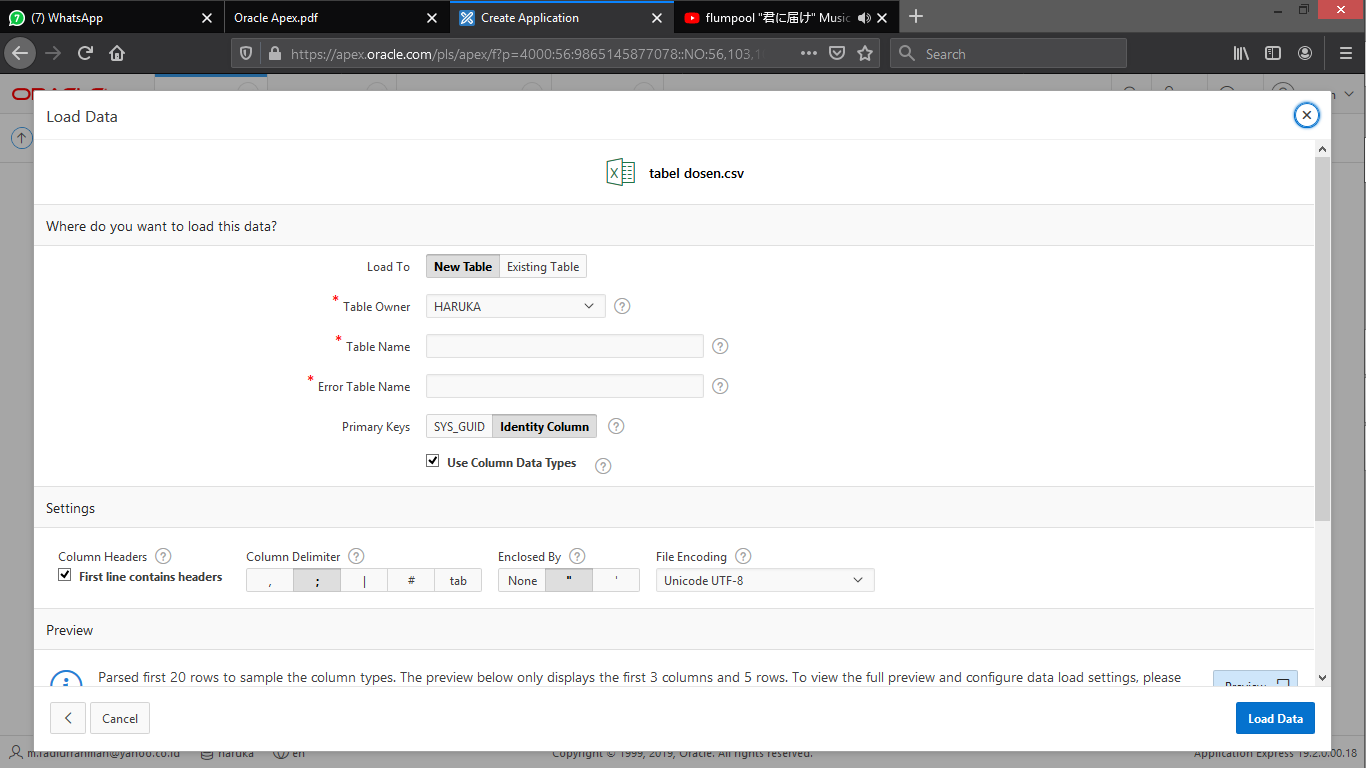
\includegraphics[scale=0.3]{src/10}
		\item Configure untuk memilih colums yang akan di load ke aplikasi, lalu click "savechange", kemudian "Load Data"\\
		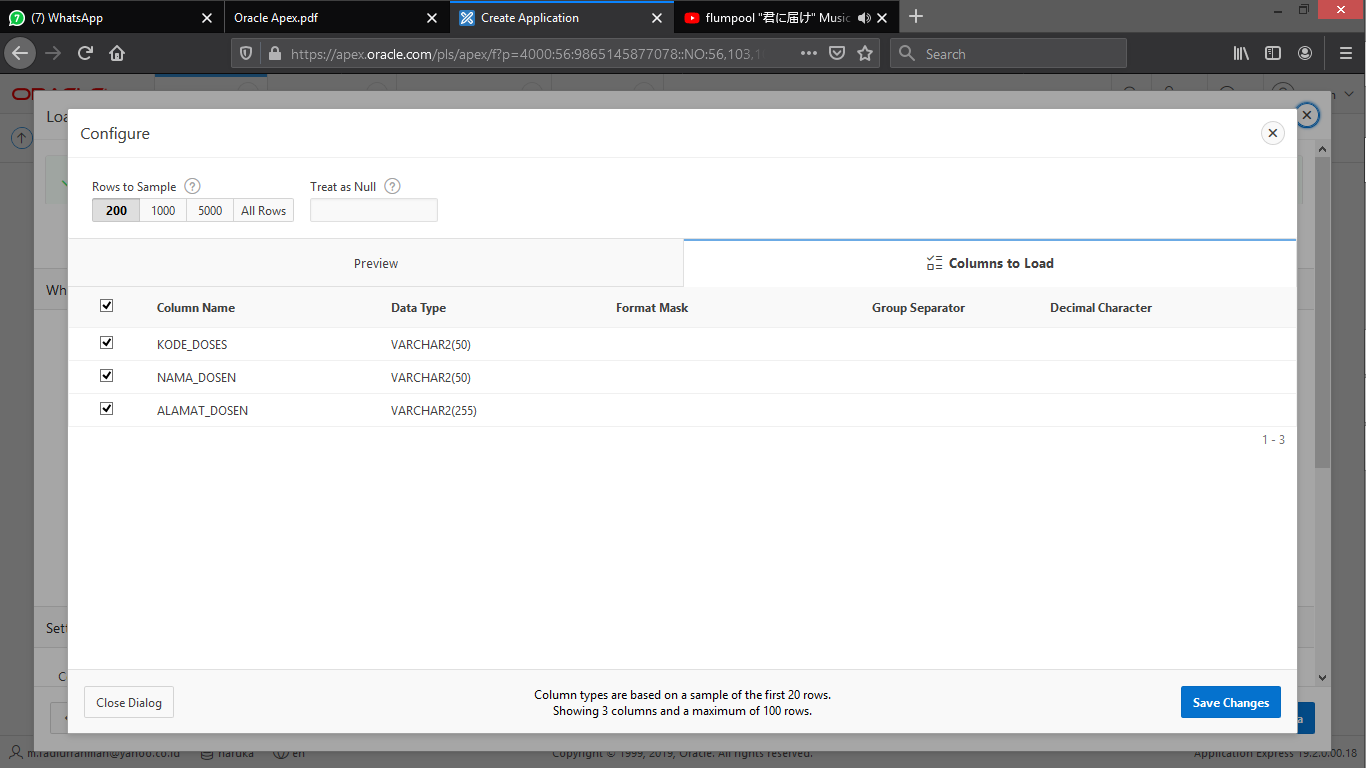
\includegraphics[scale=0.3]{src/11}
		\item Data berhasil di buat\\
		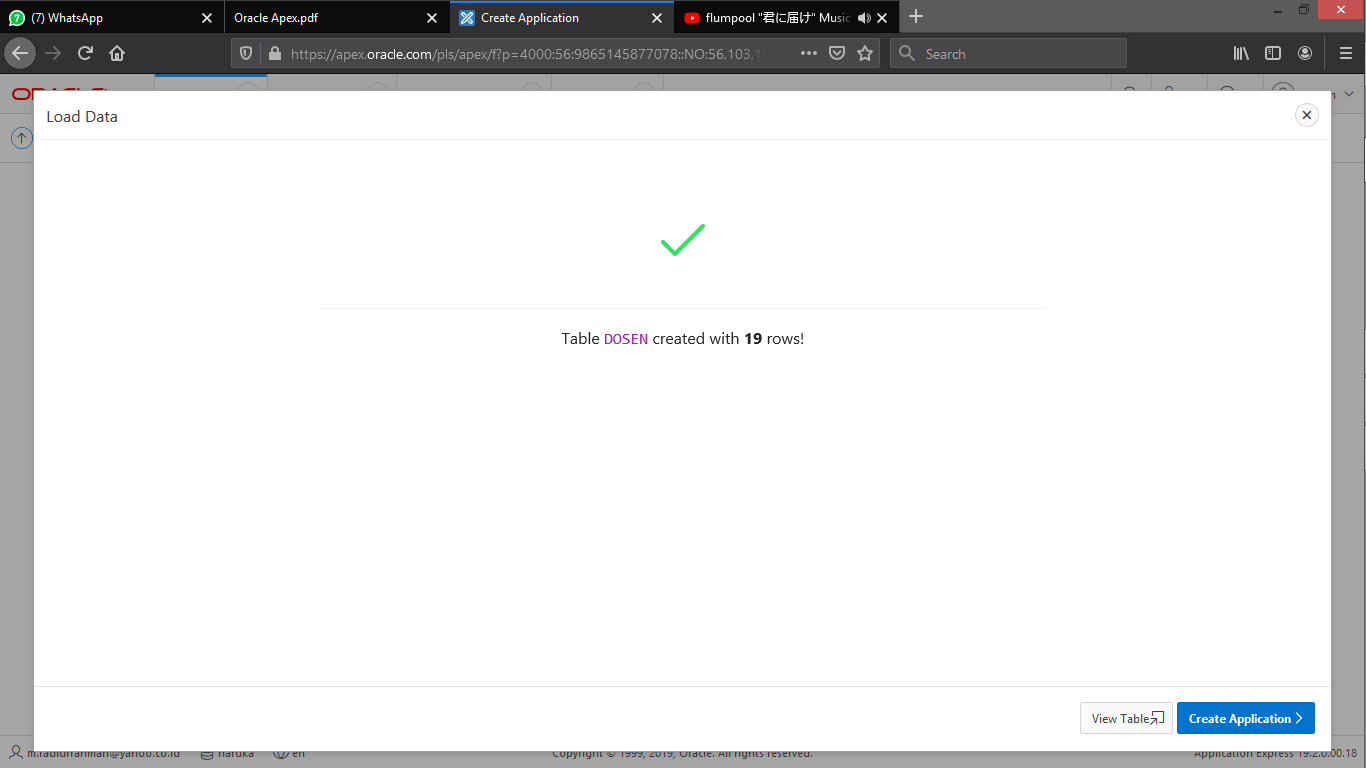
\includegraphics[scale=0.3]{src/13}
		\item Selanjutnya akan langsung di alihkan ke bagian "Create an Aplication" kemudain pilih "add page".\\
		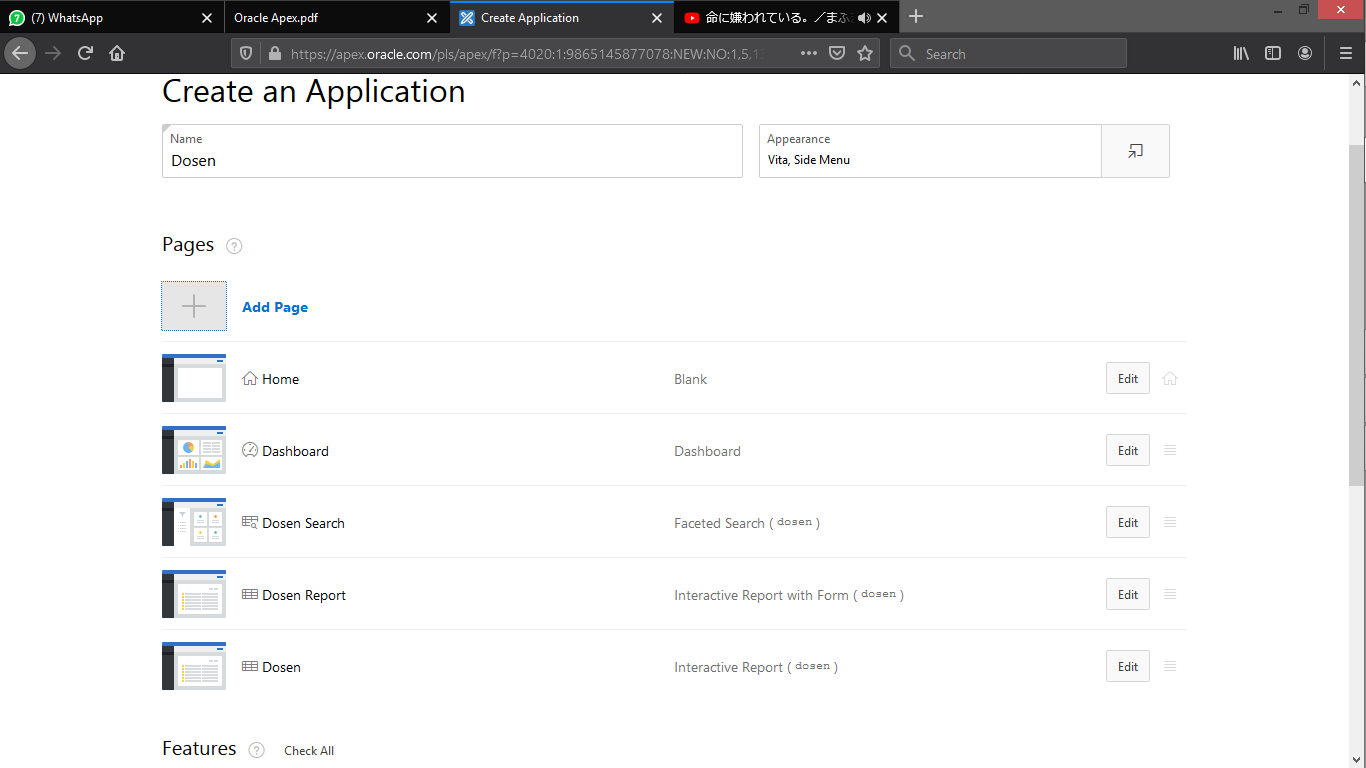
\includegraphics[scale=0.3]{src/14}
		\item Disini saya menggunakan interactive report.\\
		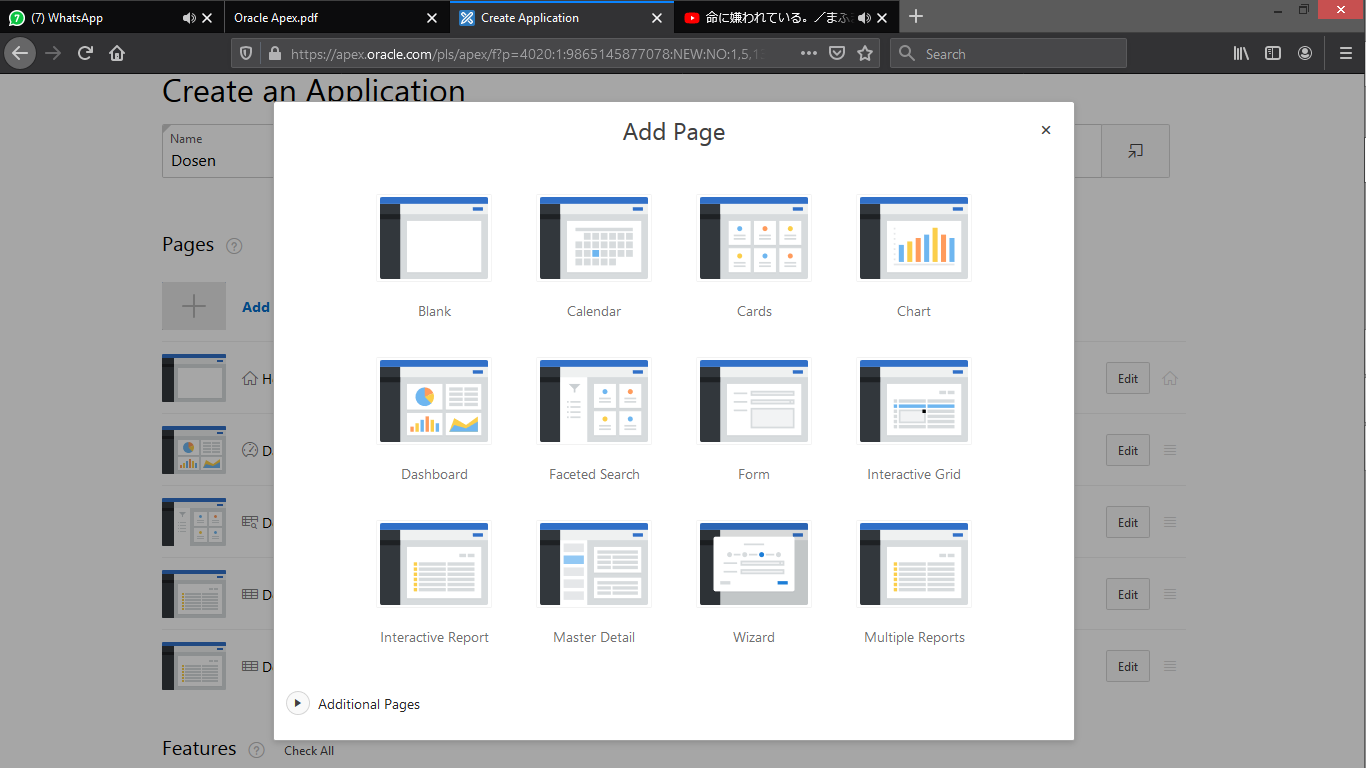
\includegraphics[scale=0.3]{src/15}
		\item masukan nama page di "page name" dan pilih data di "table and view".\\
		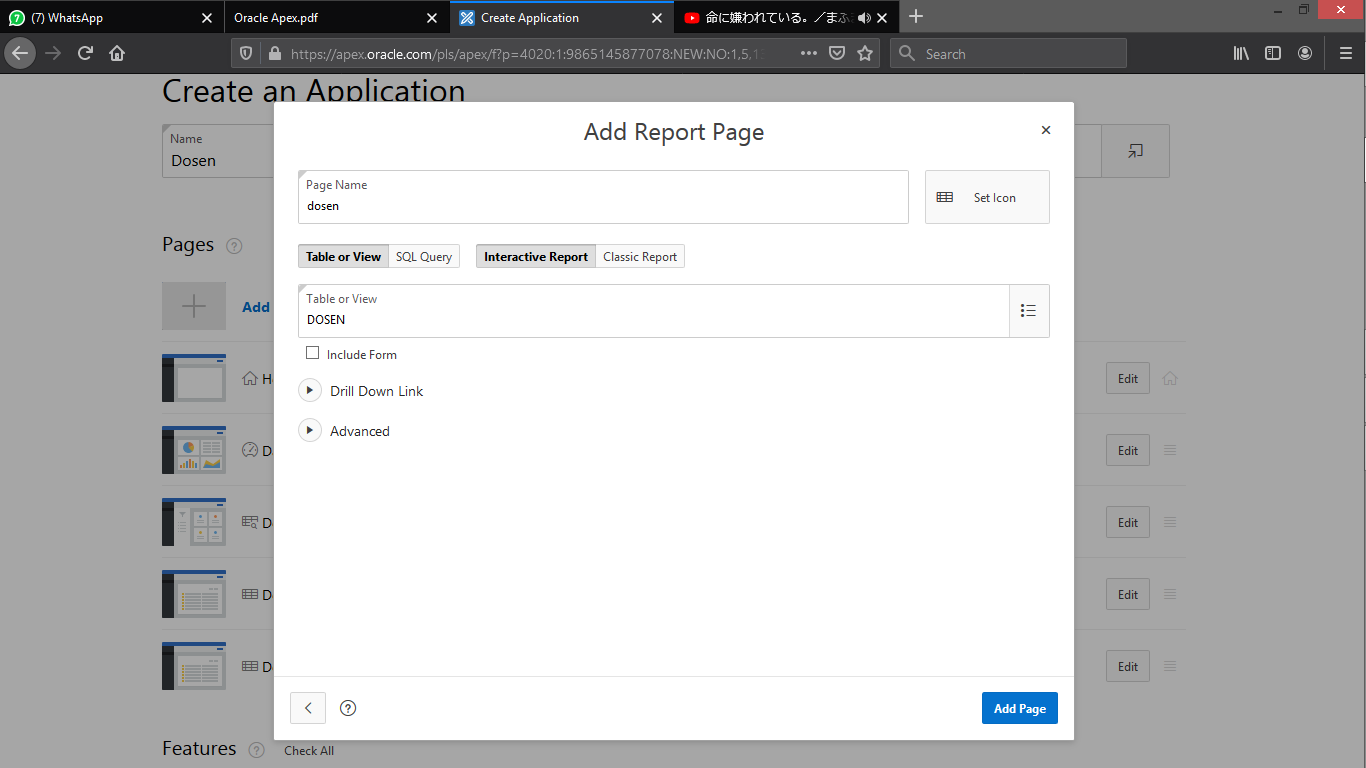
\includegraphics[scale=0.3]{src/16}
		\item kemudain jika selesai pilih "Create Aplication".\\
		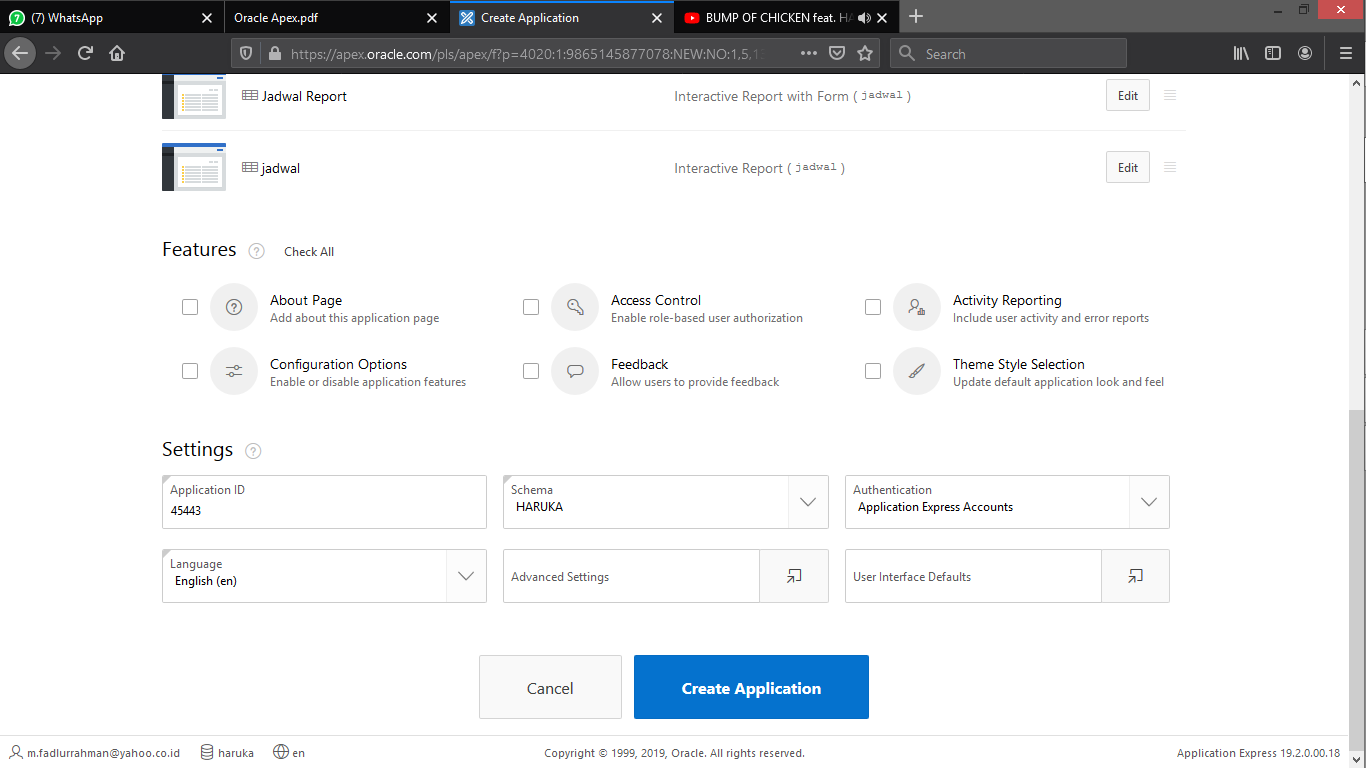
\includegraphics[scale=0.3]{src/18}
		\item selanjutnya akan langsung di alihkan ke aplikasinya, kemudian pilih "Run aplication untuk menjalankan aplikasi".\\
		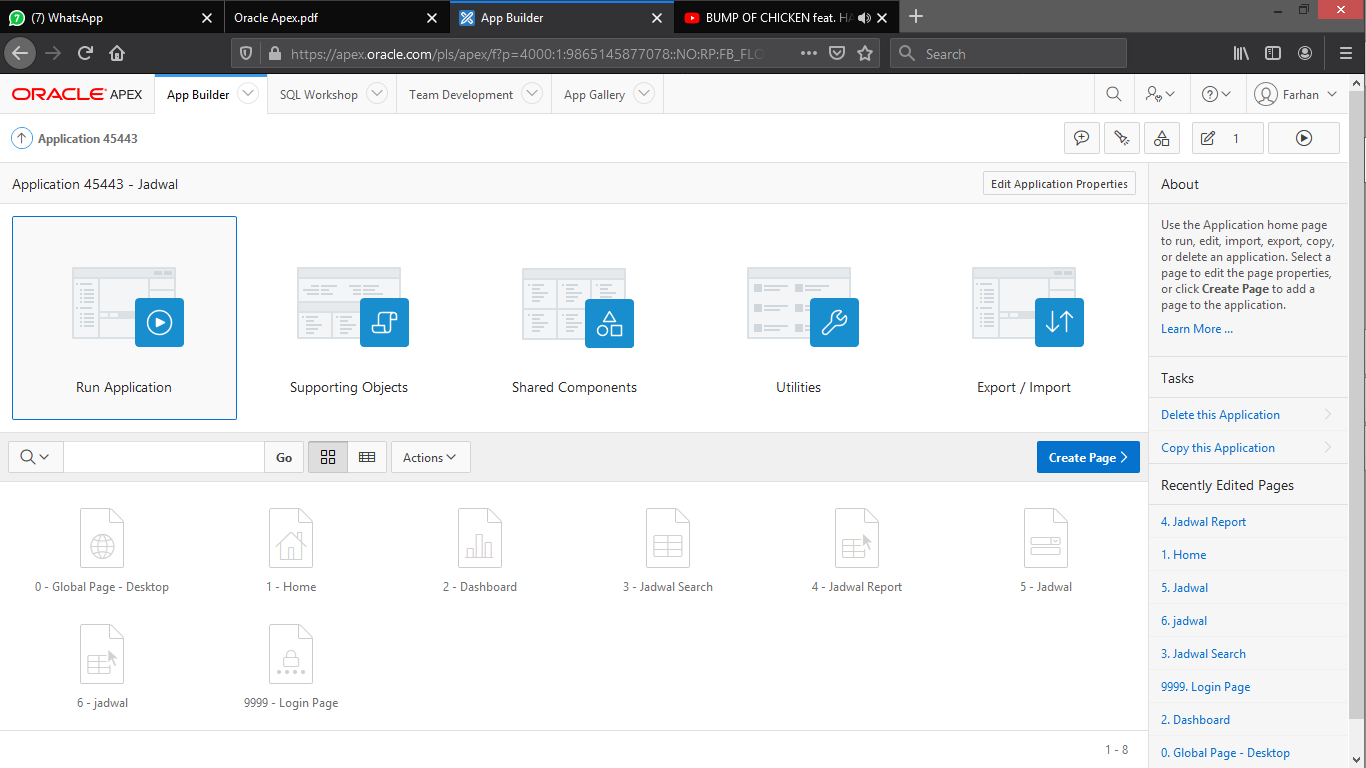
\includegraphics[scale=0.3]{src/19}
		\item aplikasi sudah jadi.\\
		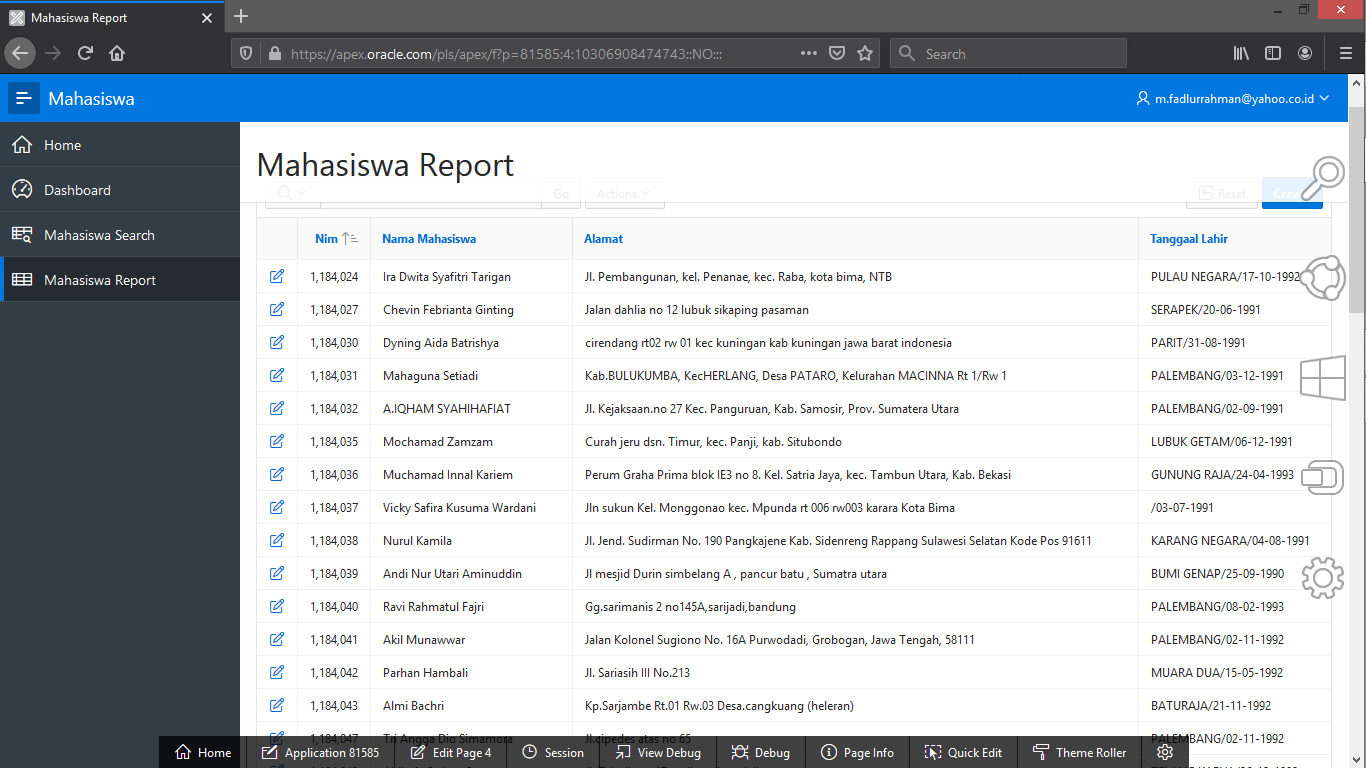
\includegraphics[scale=0.3]{src/20}
	\end{enumerate}

\section*{Email dan Link}
Email	 : m.fadlurrahman@gmail.co.id \\
Link	 : https://apex.oracle.com/pls/apex/f?p=45443:1:711768985390817:::::


\end{document}